%\renewcommand{\thefootnote}{\arabic{footnote}}
\chapter{TINJAUAN PUSTAKA}
\label{BAB2:tinjauan}
\section{Transformator Daya}

Transformator daya merupakan salah satu peralatan tenaga listrik yang berfungsi dalam mentrasmisikan daya listrik dengan cara menaikkan dan menurunkan tegangan listrik untuk mengurangi rugi-rugi daya. hal ini dikarenakan rugi-rugi daya akibat impedansi yang timbul akibat jarak transmisi yang panjang dapat dikurangi dengan menaikkan tegangan. oleh karena itu dibutuhkan transformator pada sisi pembangkitan untuk menaikkan tegangan dan pada sisi penerimaan untuk menurunkan tegangan.



\begin{equation}
  L(x,W)= \frac{1}{N}\sum\limits_{i=0}^{N} l(x_i,W)   
  \label{func:loss}
\end{equation}

\section{Indeks Kesehatan Trafo}
Dalam sistem jaringan tenaga listrik pada umumnya transformator daya yang digunakan saat beroperasi yang memiliki kondisi yang baik agar terhindar dari gangguan. kondisi sebuah transformator secara keseluruhan dapat dievaluasi dengan sebuah metode yakni indeks kesehatan transformator \cite{nurcahyanto2019analysis}. metode ini merupakan hasil kombinasi data hasil inspeksi lapangan, selama beroperasi maupun hasil pengujian transformator daya di laboratorium atau lapangan \cite{ortiz2016health}. Pengujian pada transformator daya dibagi atas pengujian elektrik, pengujian kimia, dan pengujian fisik. Metode-metode yang sering digunakan pada transformator daya diantaranya adalah \textit{Dissolve Gas Analysis} (DGA), kualitas minyak transformator, furan, faktor daya, pemantauan \textit{tap changer}, riwayat pembebanan serta data pemeliharaan \cite{jahromi2009approach}.

\subsection{\textit{Dissolve Gas Analysis} (DGA)}
DGA merupakan salah satu metode yang digunakan dalam mendeteksi adanya gangguan pada transformator daya. Dalam kondisi normal dielektrik cair pada transformator daya tidak mengalami dekomposisi dengan cepat. Namun jika terjadi adanya gangguan termal atau elektrik dapat mempercepat laju dekomposisi pada dielektrik. Proses dekomposisi dapat menghasilkan gas kontaminan yang dapat mengubah sifat kondutivitas dari isolator yang dapat memicu adanya gangguan lanjutan. Secara umum terdapat beberapa jenis gas hasil dekomposisi yang dilakukan pengecekan diantaranya adalah hidrogen, 

\section{\textit{Machine Learning}}
Machine learning merupakan salah satu metode yang digunakan dalam memodelkan pola serangkaian data untuk membuat pediksi pada input yang sama atau menyerupai 
\section{\textit{Long Short Term Memory (LSTM)}}
Pada pemodelan dengan menggunakan metode RNN secara umum memiliki kemampuan dalam membuat prediksi yang dipengaruhi oleh input sebelumnya. Namun terdapat kekurangan pada metode tersebut yakni tidak mampu mengatasi dengan  seri yang panjang. misalnya pada sebuah data \textit{time series}, RNN akan sulit mengkorelasikan antara data saat ini dengan data yang sangat lampau, akibatnya jika data yang diproses dalam rentang waktu yang lama maka RNN hanya mampu membuat prediksi yang hanya berkaitan pada waktu yang pendek. kekurangan pada RNN dikarenakan adanya \textit{vanising gradient}, yakni menghapus data yang tidak berkaitan dengan data baru yang dimasukkan. Adanya kekurangan tersebut maka dibutuhkan suatu metode baru yang dapat mengingat data lampau saat menerima input terbaru. 
LSTM merupakan salah satu turunan dari pemodelan matematis yang digunakan dalam mengenali pola serangkaian data 

kelebihan yang dimiliki LSTM dibandingkan dengan RNN dikarenakan algoritma yang digunakan terdiri dari struktur yang kompleks. Secara umum terdapat 4 bagian pada arsitektur LSTM yakni \textit{forget gate}, \textit{input gate}, \textit{Cell gate}, dan \textit{Output gate}. 
\subsection{\textit{Forget Gate}}
Pada \textit{Forget gate} merupakan bagian yang menentukan mengenai informasi pada keluaran sel sebelumnya untuk dipertahankan atau dihapus. hal ini dilakukan dengan memasukkan keluaran sel sebelumnya yang digabungkan dengan masukan baru ke dalam fungsi aktivasi sigmoid. Informasi akan dipertahankan untuk hasil dari sigmoid dengan nilai 1 dan dihapus untuk keluaran yang bernilai 0. secara matematis pada \textit{forget gate} digunakan persamaan sebagai berikut:
\begin{equation}
	\boldsymbol{f_t} = \sigma_g(\boldsymbol{W_{f}}.[\boldsymbol{h_{t-1}}, \boldsymbol{x_t}] + \boldsymbol{b_f})
	\label{func:forget}
\end{equation} 
berdasarkan persamaan~(\ref{func:forget}) dapat diketahui bahwa dengan persamaan tersebut terdapat bentuk $[\boldsymbol{h_{t-1}}, \boldsymbol{x_t}]$. Hal ini merupakan operasi penggabungan vektor yakni penggabungan baris pada $\boldsymbol{h_{t-1}}$ dengan baris pada $\boldsymbol{x_t}$
\subsection{\textit{Input Gate}}
Salah satu kelebihan LSTM adalah dapat mengingat informasi data masukan yang lama. Hal ini dikarenakan karena adanya satu bagian yang berperan dalam memperbarui memori berdasarkan informasi penting dari masukan baru. kemampuan ini diperoleh karena ada dua tahapan penting pada \textit{input gate} yakni melalui lapisan \textit{sigmoid} dan \textit{tanh}. lapisan akan memberikan keluaran berupa nilai mana saja yang harus dilakukan pembaruan pada memori sedangkan lapisan \textit{tanh} memberikan keluaran berupa calon ($\boldsymbol{\tilde{C}}$) yang ditambahkan pada memori. 
\begin{equation}
	\boldsymbol{i_t} = \sigma_i(\boldsymbol{W_{f}}.[\boldsymbol{h_{t-1}}, \boldsymbol{x_t}] + \boldsymbol{b_i})\\
	\label{func:input}
\end{equation}
\begin{equation}
	\boldsymbol{\tilde{C}} = tanh(\boldsymbol{W_{C}}.[\boldsymbol{h_{t-1}}, \boldsymbol{x_t}] + \boldsymbol{b_C})
	\label{func:C-tilde}
\end{equation}
Hasil perkalian dari dua lapisan pada \textit{input gate} akan menjadi input pada memori sebagai pembaruan. pembaruan yang terjadi dalam hanya dalam jumlah yang sedikit, oleh karena itu informasi penting pada data yang lampau akan tetap tersimpan untuk jumlah data yang banyak.
\subsection{\textit{Cell gate}}
\textit{cell gate} merupakan tempat penyimpanan informasi penting pada setiap data yang diberikan pada LSTM. \textit{cell gate} terdiri dari masukan dari \textit{forget gate} untuk mengurangi informasi yang tidak diperlukan dari semua masukan sebelumnya melalui persamaan ~(\ref{func:forget}). Kemudian ditambahkan dengan hasil perkalian dari $\boldsymbol{i_t}$ dan $\boldsymbol{\tilde{C}}$.
\begin{equation}
	\boldsymbol{C_t} = \boldsymbol{f_t}*\boldsymbol{C_{t-1}} + \boldsymbol{i_t} * \boldsymbol{\tilde{C}}
	\label{func:cell_gate}
\end{equation}
Hal utama yang perlu diperhatikan adalah bahwa pada LSTM bagian \textit{cell gate} merupakan lapisan yang saling terhubung, sehingga antar sel yang berjauhan pun dapat terintegrasi. Kondisi ini yang menjadikan LSTM dapat mengatasi permasalahan versi RNN sebelumnya yang diakibatkan adanya \textit{vanishing gradient}.
\subsection{\textit{Output Gate}}
Pada bagian akhir merupakan keluaran dari sel lstm atau dapat berupa hasil prediksi berdasarkan masukan yang diberikan. Keluaran ditentukan oleh memori $\boldsymbol{C_t}$ dan masukan yang diberikan. Hal ini dilakukan dengan memasukkan  $\boldsymbol{x_t}$ dan keluaran sebelumnya ($\boldsymbol{h_{t-1}}$) pada fungsi \textit{sigmoid}. Hasil dari fungsi \textit{sigmoid} kemudian akan memfilter nilai dari \textit{cell state} yang dapat diteruskan menuju keluaran. Sebelum dikalikan dengan hasil dari gerbang \textit{sigmoid}, \textit{cell state} terlebih dahulu melewati gerbang tanh untuk mengubah nilai pada rentang -1 sampai 1. secara matematis dapat dituliskan sebagai berikut:
\begin{equation}
	\boldsymbol{o_t} = \sigma(\boldsymbol{W_i}.[\boldsymbol{h_{t-1}}, \boldsymbol{x_t}] + \boldsymbol{b_o})
	\label{func:ouput_sigmoid}
\end{equation}
\begin{equation}
	\boldsymbol{h_t} = \boldsymbol{o_t}*tanh(\boldsymbol{C_t})
	\label{func:final_output}
\end{equation}

%Informasi ini diperoleh pada lapisan sebelumnya yakni kombinasi dari \textit{forget gate} dan \textit{input gate}. Pada dasarnya 

%\begin{align}
%	f_t &= \sigma_g(W_{f} x_t + U_{f} c_{t-1} + b_f) \\
%	i_t &= \sigma_g(W_{i} x_t + U_{i} c_{t-1} + b_i) \\
%	o_t &= \sigma_g(W_{o} x_t + U_{o} c_{t-1} + b_o) \\
%	c_t &= f_t \circ c_{t-1} + i_t \circ \sigma_c(W_{c} x_t + b_c) \\
%	h_t &= o_t \circ \sigma_h(c_t)
%\end{align}
%\lipsum[5-6]
\begin{table}[h]
    \centering
    \caption{Rata-rata loss dan accuracy Model A untuk seluruh round}
\begin{tabularx}{0.95\textwidth} { 
  | >{\centering\arraybackslash}X 
  | >{\centering\arraybackslash}X | }
 \hline
  train\_accuracy &	0.46846 \\
 \hline
  train\_loss &	2.71451 \\
 \hline
  val\_accuracy &	0.47391 \\
  \hline
  val\_loss & 2.69424 \\
  \hline
\end{tabularx}
    \label{tab:my_label} 
\end{table}

\lipsum[7]
%\begin{center}
%\begin{figure}[h]
%    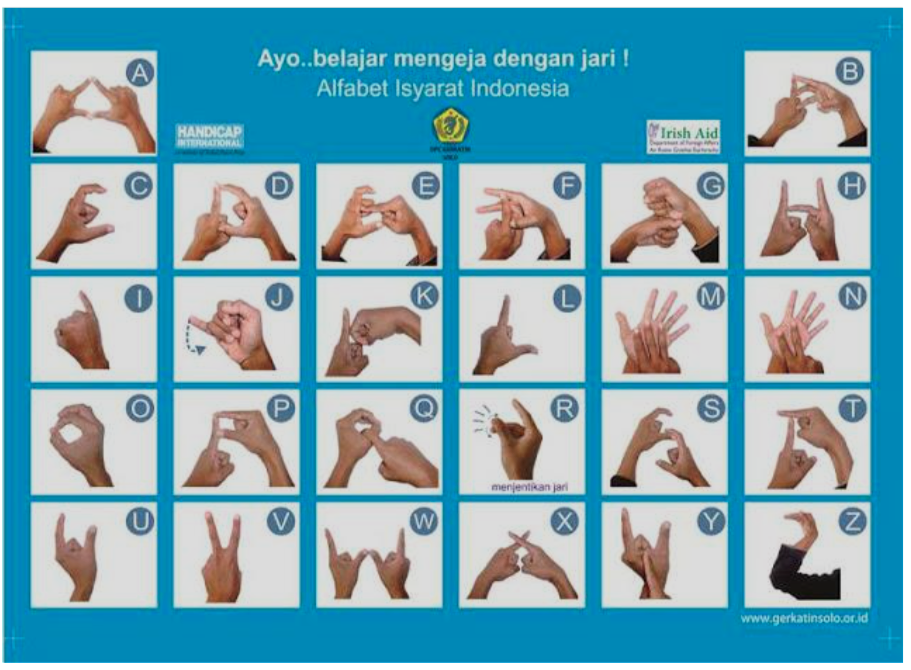
\includegraphics[width=\textwidth]{BAB-2/figures/alfabetbisindo.png}	
%	    \caption{Alfabet Bisindo (Almuharram, 2013).}
%	    \label{gambar:alfabet bisindo}
%\end{figure}
%\end{center}
Gambar \ref{gambar:alfabet bisindo} menyunjukkan sudut pandang umum yang digunakan dalam berkomunikasi menggunakan bahasa isyarat, yaitu tampak depan \citep{xiong2004_dscForSensorNetworks}. Sehingga, data gambar yang digunakan di penelitian ini juga memuat gestur Bisindo dari tampak depan, dengan persamaan~(\ref{func:loss}), dengan hasil penelitian di Bab~\ref{BAB4:hasil}.